\begin{frame}{$w_{def}(G)$ և $W_{def}(G)$ պարամետրեր}

\begin{itemize}
    \item Կամայական $G$ մուլտիգրաֆի համար $w_{def}(G)$-ով և $W_{def}(G)$-ով կնշանակենք $t$-ի ամենափոքր և ամենամեծ արժեքները, որոնց համար $G$-ն ունի $\alpha$ ճիշտ կողային ներկում $t$ գույներով և  $def(G,\alpha)=def(G)$ դեֆիցիտով:
    \item Ուսումնասիրվել է (Բուշար, Հերց, Դեսոլնյե, 2009) և (Ալտինակար, Կապորոսսի, Հերց, 2016) աշխատություններում:
    \item (Ալտինակար, Կապորոսսի, Հերց, 2016) Եթե $G$-ն ունի առնվազն երեք գագաթ, ապա $W_{def}(G)\leq 2\vert V(G)\vert -4+def(G)$:
\end{itemize}
\end{frame}


\begin{frame}[shrink]{$W_{def}(G)$ պարամետրի նոր գնահատականներ}
\begin{itemize}
\item (Հասրաթյան, Քամալյան, 1987) Եթե $G \in \mathfrak{N}$ և $G$-ն եռանկյուն չպարունակող գրաֆ է, ապա 
\begin{center}
$W(G)\leq \vert V(G)\vert -1$:
\end{center}
\end{itemize}

\begin{theorem}[3.1.3]
Եթե $G$-ն եռանկյուն չպարունակող գրաֆ է, ապա
\begin{center}
$W_{def}(G)\leq \vert V(G)\vert +def(G)-1$:
\end{center}
\end{theorem}

\begin{itemize}
\item (Հասրաթյան, Քամալյան, 1994) Եթե $G$-ն կապակցված գրաֆ է և $G\in \mathfrak{N}$, ապա
\begin{center}
$W(G)\leq 1 + \left(\mathrm{diam}(G)+1\right)\left(\Delta(G) -1\right)$:
\end{center}
% \item Եթե $G$-ն կապակցված երկկողմանի գրաֆ է և $G\in \mathfrak{N}$, ապա $W(G)\leq \mathrm{diam}(G)\left(\Delta(G) -1\right) +1$ (Հասրաթյան, Քամալյան, 1994)
\end{itemize}


\begin{theorem}[3.1.6]
Եթե $G$-ն կապակցված գրաֆ է, ապա
\begin{center}
$W_{def}(G)\leq
1+def(G)+(\mathrm{diam}(G)+1)\left(\Delta(G)-1\right)$:
\end{center}
\end{theorem}
\end{frame}

\begin{frame}{$w_{def}(G)$ պարամետրի նոր գնահատական}{կախված նվազագույն աստիճանից}

\begin{theorem}[3.1.7]
Եթե $G$-ն չունի կատարյալ զուգակցում, ապա
\begin{center}
$w_{def}(G)\geq 2\delta(G)-def(G)$:
\end{center}
\end{theorem}

Այս թեորեմը ընդհանրացնում է Բուշարի, Հերցի և Դեսոլնյեի կողմից ստացված երկու արդյունքները:
\begin{hide}

\begin{corollary}
\label{c3_wdef_odd}\cite{BouchardHertzDesaulniers} Եթե $G$-ն կենտ թվով գագաթներ ունեցող գրաֆ է, ապա
\begin{center}
$w_{def}(G)\geq 2\delta(G)-def(G)$:
\end{center}
\end{corollary}

\begin{corollary}
\label{c3_wdef_odd_regular}\cite{BouchardHertzDesaulniers} Եթե $G$-ն կենտ թվով գագաթներ ունեցող $r$-համասեռ գրաֆ է և $def(G)=\frac{r}{2}$, ապա
$w_{def}(G)\geq \frac{3r}{2}$:
\end{corollary}
\end{hide}
\end{frame}

\begin{frame}{$w_{def}(G)$ և $W_{def}(G)$ պարամետրեր}

\begin{itemize}
    \item Քամալյանը (1990) ապացուցել է, որ կամայական $l\in \mathbb{N}$ թվի համար գոյություն ունի $G$ գրաֆ այնպիսին, որ $G\in \mathfrak{N}$ և $W(G)-w(G)\geq l$:
\end{itemize}

\begin{theorem}[3.1.10]
Ցանկացած $l\in \mathbb{N}$ թվի համար գոյություն ունի $G$ գրաֆ այնպիսին, որ $def(G)>0$ և $W_{def}(G)-w_{def}(G)\geq l$:
\end{theorem}
\begin{hide}

\begin{figure}[t!]
\centering
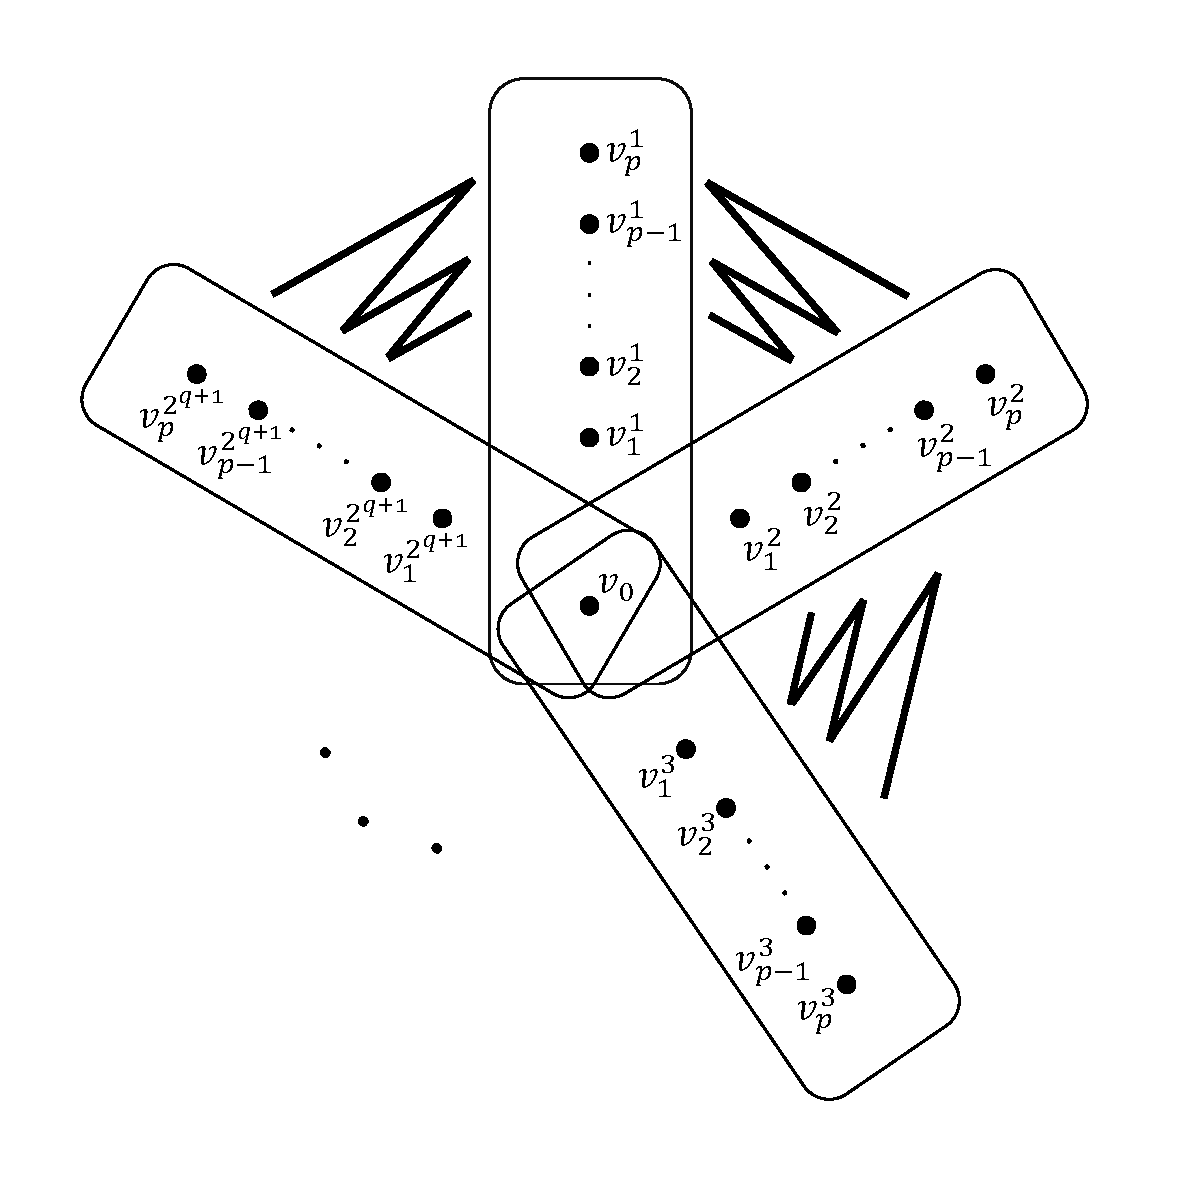
\includegraphics[width=0.7\textwidth]{figures/complete-graph-edges.pdf}
\caption{$K_{p2^{q+1}+1}$ գրաֆի գագաթները բաժանում ենք $2^{q+1}$ խմբերի այպես, որ կամայական երկու խմբի հատումը $v_0$ գագաթն է:}
\label{complete-graph}
\end{figure}
\end{hide}
\end{frame}

\begin{frame}{$w_{def}(G)$ և $W_{def}(G)$ պարամետրեր}
\begin{itemize}
    \item Հասրաթյանը և Քամալյանը ցույց էին տվել, որ եթե $G$-ն համասեռ մուլտիգրաֆ է, իսկ $w(G) \leq t \leq W(G)$, ապա $G$-ն ունի միջակայքային $t$-ներկում:
\end{itemize}

\begin{theorem}[3.1.11]
Դիցուք $\alpha_0$-ն $G$ համասեռ մուլտիգրաֆի ճիշտ ներկում է $t_0$ գույներով, իսկ $D \subseteq V(G)$ նրա գագաթների որևէ ենթաբազմություն է: Եթե կամայական $v \in V(G) \setminus D$ գագաթի համար $def(v,\alpha_0)=0$, ապա ցանկացած $t$ թվի համար, $\overline{S}(D,\alpha_0) - \underline{S}(D,\alpha_0) + 1 \leq t \leq t_0$, $G$-ն ունի $\alpha$ ճիշտ ներկում $t$ գույներով այնպես, որ $def(v,\alpha) = def(v,\alpha_0)$ կամայական $v\in V(G)$ գագաթի համար:
\end{theorem}
\end{frame}

\begin{frame}{Կենտ թվով գագաթներով լրիվ գրաֆներ}
\begin{itemize}
    \item (Գիառո, Կուբալ, Մալաֆիյսկի, 2001)
    Եթե $n\in \mathbb{N}$, ապա $def(K_{2n+1})=n$:    
    \item (Բուշար, Հերց, Դեսոլնյե, 2009) Եթե  $n\in \mathbb{N}$, ապա $w_{def}(K_{2n+1})=3n$:    
\end{itemize}

\begin{theorem}[3.1.12]
Դիցուք $n=p2^q$, որտեղ $p$-ն կենտ է, իսկ $q \in \mathbb{Z}_{\geq 0}$: 

Կամայական $t$ թվի համար,
\begin{center}
$3n \leq t \leq 3n + \frac{p-1}{2}$,
\end{center} $K_{2n+1}$-ը ունի $\alpha$ ճիշտ ներկում $t$ գույներով այնպես, որ $def(K_{2n+1},\alpha)=n$:
\end{theorem}
\end{frame}
